\documentclass{standalone}
\usepackage{tikz}
\usepackage{xcolor-solarized}
\usetikzlibrary{positioning}

\newcommand\commit[2][]{\node[commit, #1] (#2) { \Large \texttt{#2} };}
\newcommand\commitWork[2][]{\node[commit, fill=solarized-blue!50, #1] (#2) { \Large \texttt{#2} };}
\newcommand\ghost[1]{\coordinate (#1);}
\newcommand\connect[2]{\path[thick] (#1) to[out=0, in=180] (#2);}

\begin{document}
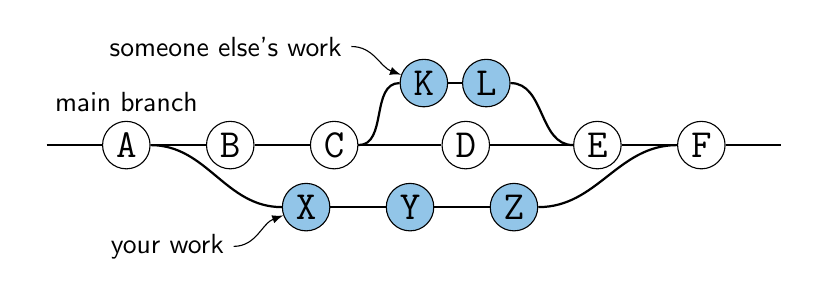
\begin{tikzpicture}

\tikzset{every node}=[font=\sffamily]

\tikzstyle{commit}=[draw, circle, fill=white, inner sep=0.2em, minimum size=1em]
\tikzstyle{every path}=[draw]

\node[] (start) {};
\commit[right=2em of start]{A};
\commit[right=2em of A]{B};
\commit[right=2em of B]{C};
\commit[right=3em of C]{D};
\commit[right=3em of D]{E};
\commit[right=2em of E]{F};
\node[right=2em of F] (end) {};

\connect{start}{A};
\connect{A}{B};
\connect{B}{C};
\connect{C}{D};
\connect{D}{E};
\connect{E}{F};
\connect{F}{end};

\node[above=0em of A] (MB) {main branch};

\commitWork[above right=1em and 2em of C]{K};
\commitWork[right=0.5em of K]{L};

\connect{C}{K};
\connect{K}{L};
\connect{L}{E};

\node[above left=0em and 2em of K] (SEW) {someone else's work};
\draw[-latex] (SEW) to[out=east, in=160] (K);

\commitWork[below right=1em and 1.5em of B]{X};
\commitWork[right=2em of X]{Y};
\commitWork[right=2em of Y]{Z};

\connect{A}{X};
\connect{X}{Y};
\connect{Y}{Z};
\connect{Z}{F};

\node[below left=0em and 2em of X] (YW) {your work};
\path[-latex] (YW) to[out=east, in=200] (X);
%\gittag[vA]{vA}{above=of A}{A};

\end{tikzpicture}
\end{document}
